\documentclass[a4paper]{article}
% Start Preamble
\usepackage[utf8]{inputenc}
\usepackage{fullpage}
\usepackage[english]{babel}
\usepackage{color}
\usepackage{url}
\usepackage{standalone}
\usepackage{parskip} % Package to tweak paragraph skipping
\usepackage{hyperref}
\usepackage{amsmath,amssymb}
\usepackage[version=4]{mhchem} 
\usepackage{bm}
\usepackage{verbatim}
\usepackage{subfig}
\graphicspath{ {./Figures/} }

\definecolor{burntorange}{cmyk}{0,0.52,1,0}
\definecolor{springgreen}{cmyk}{1,0,0.8,0}

\title{Reflection and Refraction}
\author{Lauren Shriver}
\date{September 26 2018}
% End Preamble
\begin{document}
\maketitle

\section*{Specular and Diffuse Relection}
There are two types of reflection: specular reflection and diffuse reflection. 
\subsection*{Aside}
There are two light rays we need to specify when discussing light reflection:
\begin{enumerate}
    \item \textbf{Incidence ray} = the light ray approaching a reflective surface
        \begin{itemize}
            \item The \textcolor{burntorange}{\textbf{angle of incidence} $\theta_i$} is the angle between the axis perpendicualr to the reflective surface and the incidence ray 
        \end{itemize}
    \item \textbf{Reflective ray} = the resulting light ray that appears to "bounce" off the reflective surface at the point where the incidence ray collides with the surface 
        \begin{itemize}
            \item The \textcolor{springgreen}{\textbf{angle of reflection} $\theta_r$} is the angle between the axis perpendicualr to the reflective surface and the reflective ray 
        \end{itemize}
\end{enumerate}
\begin{figure}[htp!]
        \centering
        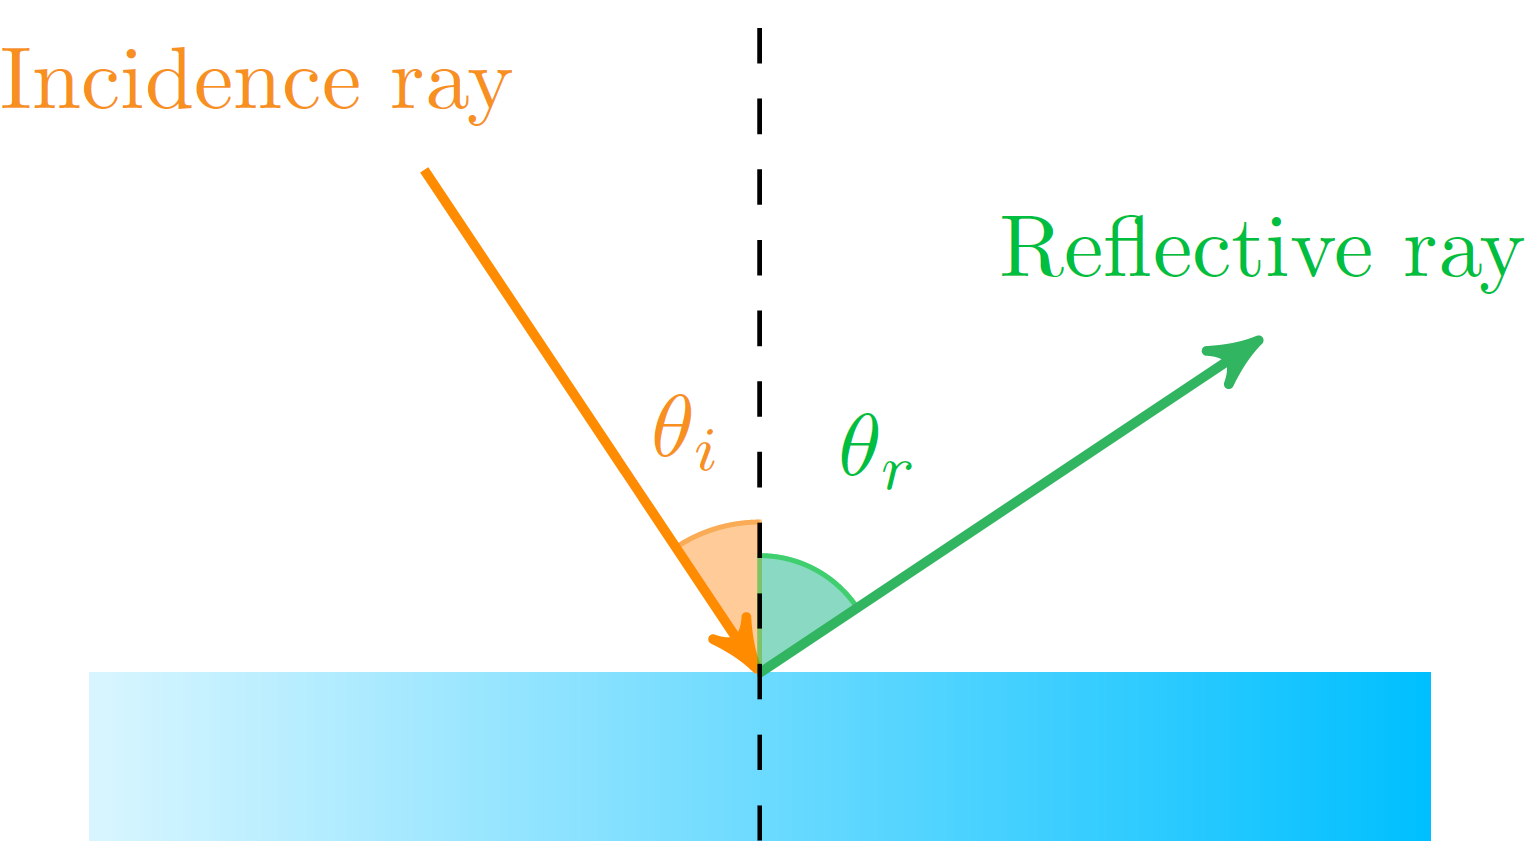
\includegraphics[width=7cm]{incidence_refractive.png}
        \caption{An incidence ray (orange) and its corresponding reflective ray (green). $\theta_i$ denotes the angle of incidence and $\theta_r$ denotes the angle of reflection.}
        \label{fig:inci_refrac}
\end{figure}
\subsection*{Specular Reflection}
The defining property of \textbf{specular reflection} is $\theta_i = \theta_r$ (as shown in figure \ref{fig:spec_reflec}). 
\begin{figure}[htp!]
        \centering
        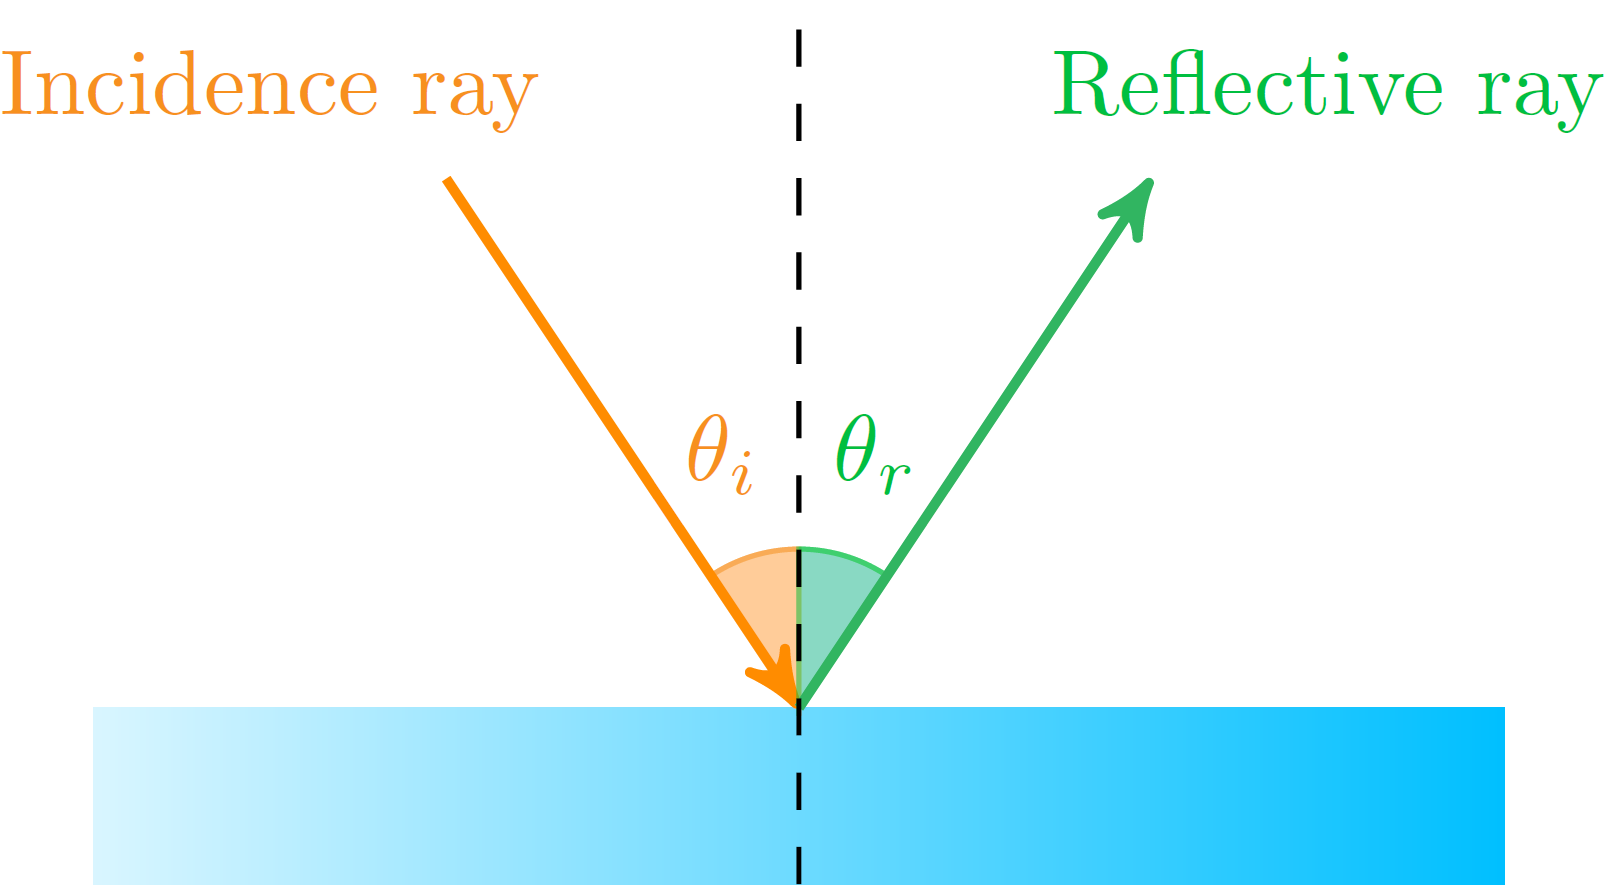
\includegraphics[width=7cm]{specular_reflection.png}
        \caption{Specular Reflection (Note: both rays are oriented such that $\theta_i = \theta_r$)}
        \label{fig:spec_reflec}
\end{figure}
\section*{Relection vs. Refraction}
\end{document}
